\section{Exercise 3}
The following system of equations
\begin{subequations}
    \begin{equation}
        2x + 3y = 4
        \label{eq:1}
    \end{equation}
    \begin{equation}
        x + 2y = 5
        \label{eq:2}
    \end{equation}
    can easily be solve by hand. First solve for $x$ in terms of $y$ in
    Eq.~(\ref{eq:2}), 
    \begin{equation}
        x = 5-2y
        \label{eq:3}
    \end{equation}
    Next substitute $x$ into Eq.~(\ref{eq:1}) to obtain a value for $y$,
    namely
    \begin{equation}
        2(-5-2y) + 3y = 4 \rightarrow y = 6
    \end{equation}
    Thus
    \begin{empheq}[box=\widefbox]{equation}
        x = -7
    \end{empheq}
    \begin{empheq}[box=\widefbox]{equation}
        y = 6
    \end{empheq}
\end{subequations}
Furthermore, the solution can be verified by solving for $y$ in both
equations and plotting both curves and observing their intersection point,
as shown in Fig~(\ref{fig:exercise-3}).  

\begin{figure}[H]
    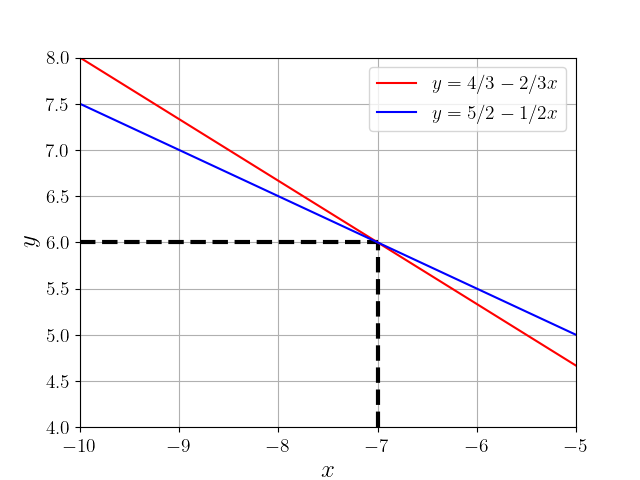
\includegraphics[height=3.0in]{media/exercise-3.png}
    \caption{Verification plot for Exercise 3}
    \label{fig:exercise-3}
\end{figure}

The following python commands were used in to verify the solution.
\lstdefinestyle{mystyle}{
    backgroundcolor=\color{backcolour},   
    commentstyle=\color{codegreen},
    keywordstyle=\color{magenta},
    numberstyle=\tiny\color{codegray},
    stringstyle=\color{codepurple},
    basicstyle=\ttfamily\footnotesize,
    breakatwhitespace=false,         
    breaklines=true,                 
    captionpos=b,                    
    keepspaces=true,                 
    numbers=left,                    
    numbersep=5pt,                  
    showspaces=false,                
    showstringspaces=false,
    showtabs=false,                  
    tabsize=2
}

\lstset{style=mystyle}
\lstinputlisting[language=Python]{latex-inputs/exercise-3.py}

